\documentclass{book}
\usepackage{html}
\usepackage{fancyheadings}
\usepackage{graphicx}

\newcommand{\gnutls}{{\emph{GNUTLS}} }
\newcommand{\tls}{{\emph{TLS}} }
\newcommand{\ssl}{{\emph{SSL}} }
\newcommand{\HRule}{\rule{\linewidth}{0.4mm}}


\begin{document}

\pagenumbering{roman}

\thispagestyle{empty}

\setlength{\parindent}{0mm}

\setlength{\parskip}{0mm}

 {\Huge GNUTLS\\[.1mm]}
 \HRule
 \begin{flushright}
  a Transport Layer Security Library
 \end{flushright}

 \vspace*{\stretch{3}}

 {\Large By Nikos Mavroyanopoulos and Fabio Fiorina\\[.1mm]}
 \HRule
 
\newpage

\vspace*{\stretch{2}}

\begin{center}
\par
Permission is granted to copy, distribute and/or modify this
document under the terms of the GNU Free Documentation License,
Version 1.1 or any later version published by the Free Software
Foundation; with no Invariant Sections, no Front-Cover Texts and
no Back-Cover Texts.  A copy of the license is included in the
chapter entitled "GNU Free Documentation License".
\end{center}



\tableofcontents
\newpage
\pagenumbering{arabic}
\pagestyle{fancy}

\chapter{The Library}
\section{Introduction}
\par
\gnutls{} is a portable library which implements the \tlsI{} and 
\sslIII{} protocols.
\tls{} stands for 'Transport Layer Security' and is the sucessor of \ssl{}, 
the Secure Sockets Layer protocol designed by Netscape. 

\tlsI{}\footnote{described in {\it RFC 2246}} is an Internet protocol,
defined by {IETF}\footnote{IETF or Internet Engineering Task Force 
is a large open international community of network
designers, operators, vendors, and researchers concerned with the evolution of 
the Internet architecture and the smooth operation of the Internet. It is open to any interested individual.}, 
that provides confidentiality, and authentication layers over any reliable
transport layer.

\par
\gnutls{} implements the above
protocols in a reentrant way. This allows multiple threads of
execution, without the need for critical sections and locks. See
\htmladdnormallink{http://www.gnutls.org/}{http://www.gnutls.org/}
and \htmladdnormallink{http://www.gnu.org/software/gnutls/}{http://www.gnu.org/software/gnutls/} 
for updated versions of the \gnutls{} software and this document.

\par
Currently \gnutls{} implements:
\begin{itemize}
 \item the \tlsI{} and \sslIII{} protocols, without any weak algorithms\footnote{
There are ciphersuites in \tlsI{} that are considered weak. These
ciphersuites are deliberately weak in order to be able to export encryption
software from some countries.}
 \item {\bf X.509} Public Key Infrastructure.
 \item {\bf OpenPGP} Public Key Infrastructure.
 \item {\bf SRP} for \tls{} authentication.
 \item \tls{} {\bf Extension mechanism}.
\end{itemize}

\newpage
\section{TLS layers}

\tlsI{} is a layered protocol, and consists of the Record Protocol,
the Handshake Protocol and the Alert Protocol. The Record Protocol
is to serve all other protocols and is above the transport layer.
The Record protocol offers symmetric encryption, and data authenticity.
In \gnutls{} the record protocol is accessed using the 
\hyperref{gnutls\_record\_read()}{gnutls\_record\_read() (see Section }{)}{gnutls_record_read} and
\hyperref{gnutls\_record\_write()}{gnutls\_record\_write() (see Section }{)}{gnutls_record_write}
functions.

\par
The Alert protocol offers some signaling to the other protocols. It can
help informing the peer for the cause of failures and other error
conditions.
\hyperref{gnutls\_alert\_send()}{gnutls\_alert\_send() (see Section }{)}{gnutls_alert_send} and
\hyperref{gnutls\_alert\_send\_appropriate()}{gnutls\_alert\_send\_appropriate() (see Section }{)}{gnutls_alert_send_appropriate} 
functions.

\par 
The Handshake protocol is responsible for the initial key exchange,
and authentication. See \hyperref{figure}{figure }{}{fig:cert} for the
protocol layering in TLS. The handshake protocol in \gnutls{} is accessed
with the 
\hyperref{gnutls\_handshake()}{gnutls\_handshake() (see Section }{)}{gnutls_handshake} function.

\begin{figure}[hbtp]
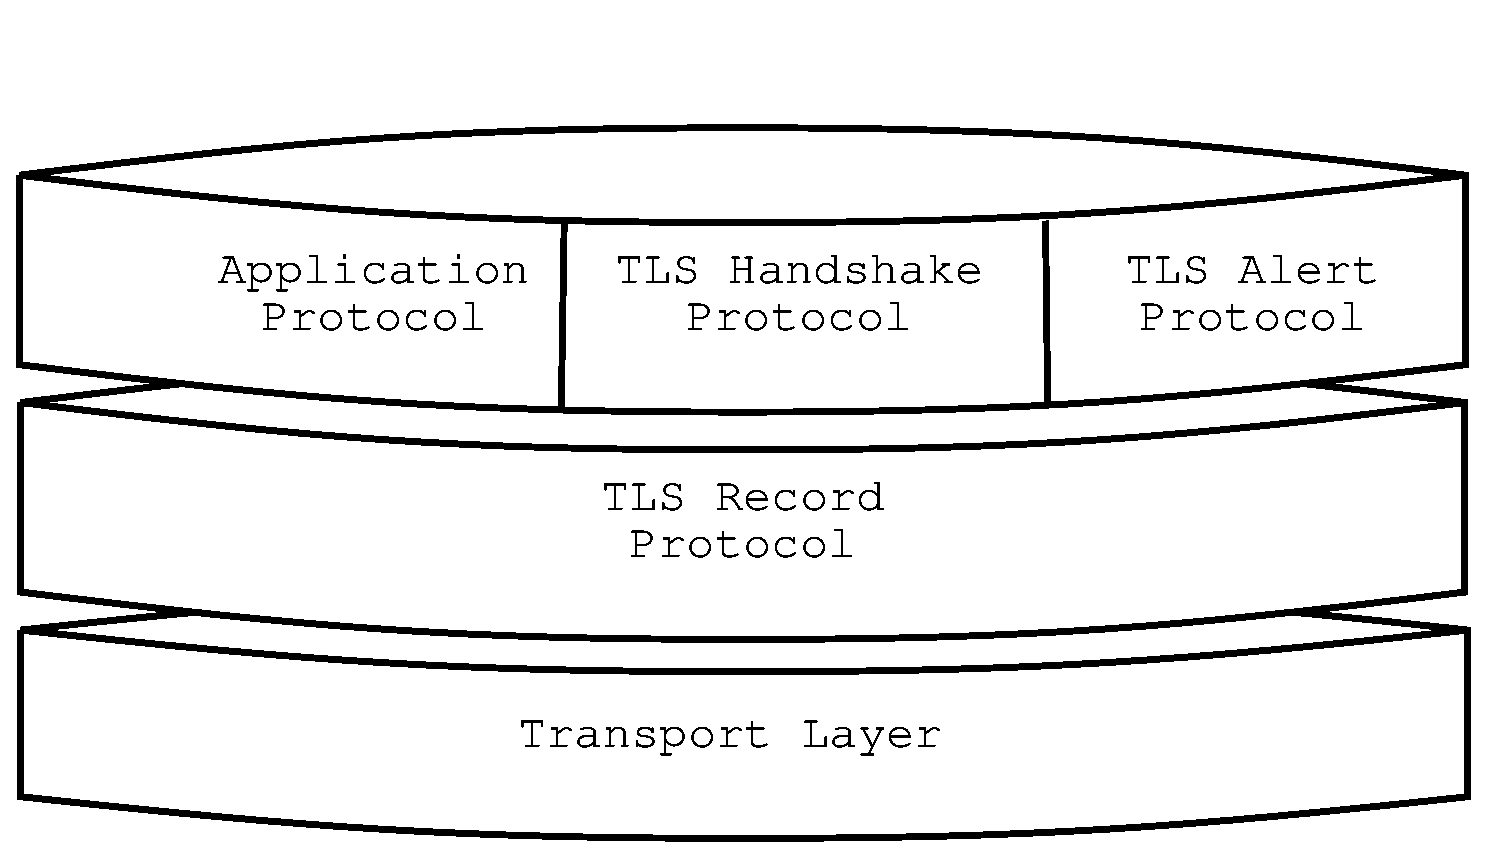
\includegraphics{layers}
\label{fig:layers}

\end{figure}


\addvspace{1.5cm}



\section{Transport Layer}
\par
\gnutls can be used above any transport layer. To do this you will only 
need to set up the 
\hyperref{gnutls\_transport\_set\_push\_function()}{gnutls\_transport\_set\_push\_function() (see Section }{
for more information)}{gnutls_transport_set_push_function} and
\hyperref{gnutls\_transport\_set\_pull\_function()}{gnutls\_transport\_set\_pull\_function() (see Section }{
for more information)}{gnutls_transport_set_pull_function}
functions. These functions will then be used by gnutls in order to send and receive data.
The functions specified should return -1 on error and should set errno appropriately.
\gnutls supports EINTR and EAGAIN errno values. These values are
usually used in non blocking IO and interrupted system calls.
The corresponding values (GNUTLS\_E\_INTERRUPTED, GNUTLS\_E\_AGAIN) 
will be returned to the caller of the gnutls function. \gnutls functions
can be resumed (called again), if any of these values is returned.
\par
By default (if none of the above functions are not called), gnutls will use
the berkeley sockets functions recv() and send(). In this case
gnutls will use some hacks in order for select() to work, thus
making easy to add {\emph TLS} support to existing servers.




\section{The TLS record protocol\index{TLS protocols!Record}}

The Record protocol is the secure communications provider. It's purpose
is to encrypt, authenticate and --optionally-- compress packets.
The following functions are available:
\par
\begin{itemize}
\item \printfunc{gnutls_record_send}{gnutls\_record\_send}:
to send a record packet (with application data).
\item \printfunc{gnutls_record_recv}{gnutls\_record\_recv}:
to receive a record packet (with application data).
\end{itemize}

As you may have already noticed, the functions which access the Record protocol,
are quite limited, given the importance of this protocol in \tls{}.
This is because the Record protocol's parameters are all set by
the Handshake protocol (see section \ref{handshake} on page \pageref{handshake}).
\par
The Record protocol initially starts with NULL parameters, which means
no encryption, and no MAC is used. Encryption and authentication begin
just after the handshake protocol has finished.

\subsection{Encryption algorithms used in the record layer}
\index{Symmetric encryption algorithms}
Confidentiality in the record layer is achieved by using symmetric block 
encryption algorithms like {\bf 3DES}, {\bf AES\footnote{AES or Advanced 
Encryption Standard is actually the RIJNDAEL algorithm. This is the
algorithm that replaced DES.}}, or
stream algorithms like {\bf ARCFOUR\_128\footnote{ARCFOUR\_128 is a compatible
algorithm with RSA's RC4 algorithm, which is considered to be a trade secret.}} See \hyperref{fig:ciphers}{figure }{}{fig:ciphers} for a complete list. 
Ciphers are encryption algorithms that use a single (secret) key
to encrypt and decrypt data. Block algorithms in TLS also provide protection
against statistical analysis of the data. \gnutls{} makes use of this property
thus, if you're using the \tlsI{} protocol, a random number of blocks will be
appended to the data. This will prevent eavesdroppers from guessing the 
actual data size.

\begin{figure}[hbtp]
\begin{tabular}{|l|p{9cm}|}

\hline
3DES\_CBC & 3DES\_CBC is the DES block cipher algorithm used with triple
encryption (EDE). Has 64 bits block size and is used in CBC mode.
\\
\hline
ARCFOUR\_128 & ARCFOUR is a fast stream cipher.
\\
\hline
ARCFOUR\_40 & This is the ARCFOUR cipher that is fed with a 40 bit key,
which is considered weak.
\\
\hline
AES\_CBC & AES or RIJNDAEL is the block cipher algorithm that replaces 
the old DES algorithm. Has
128 bits block size and is used in CBC mode. This is not officially
supported in TLS.
\\
\hline
\end{tabular}
\caption{Supported cipher algorithms}
\label{fig:ciphers}
\end{figure}



\addvspace{1.5cm}

\begin{figure}[hbtp]
\begin{tabular}{|l|p{9cm}|}

\hline
MAC\_MD5 & MD5 is a cryptographic hash algorithm designed by Ron Rivest. Outputs 128 bits of data.
\\
\hline
MAC\_SHA & SHA is a cryptographic hash algorithm designed by NSA. Outputs 160 bits of data.
\\
\hline
MAC\_RMD160 & RIPEMD is a cryptographic hash algorithm developed in the framework
of the EU project RIPE. Outputs 160 bits of data.
\\
\hline
\end{tabular}
\caption{Supported MAC algorithms}
\index{MAC algorithms}
\label{fig:mac}
\end{figure}



\subsection{Compression algorithms used in the record layer}
\index{Compression algorithms}
The TLS' record layer also supports compression. The algorithms
implemented in \gnutls{} can found in figure \ref{fig:compression}.
All the algorithms should be considered as \gnutls' extensions, and
should be advertised only when the peer is known to have a compliant client,
to avoid interoperability problems.
\par
The included algorithms perform really good when text, or other
compressable data are to be transfered, but offer nothing on already 
compressed data, such as compressed images, zipped archives etc.
These compression algorithms, may be useful in high bandwidth TLS tunnels,
and in cases where network usage has to be minimized. As a drawback, 
compression increases latency.

\begin{figure}[hbtp]
\begin{tabular}{|l|p{9cm}|}

\hline
ZLIB & ZLIB compression, using the deflate algorithm.
\\
\hline
LZO & LZO is a very fast compression algorithm. This algorithm is only
available if the \gnutlse{} library has been initialized.
\\
\hline
\end{tabular}
\caption{Supported compression algorithms}
\label{fig:compression}
\end{figure}




\subsection{Weaknesses and countermeasures}
\index{TLS protocols!Record}

Some weaknesses that may affect the security of the Record layer have been
found in \tlsI{} protocol. These weaknesses can be exploited by active attackers,
and exploit the facts that \tls{} 
\begin{enumerate}
\item has separate alerts for ``decryption\_failed'' and ``bad\_record\_mac''
\item the decryption failure reason can be detected by timing the responce time
\item the IV for CBC encrypted packets is the last block of the previous encrypted packet
\end{enumerate}

\gnutls{} implements all the known counter-measures for these attacks. For the first
two cases, \gnutls{} does only have one error code for both of the decryption failures,
and processes the message normaly even if a padding error occured. This avoids
both of these attacks.
For the latter, an empty record can be sent before every record packet, and this is
believed to avoid the known attacks in CBC encrypted packets. See the function
\printfunc{gnutls_record_set_cbc_protection}{gnutls\_record\_set\_cbc\_protection}
for more information.

For a detailed discussion see the archives of the TLS Working Group mailing list
and the paper \cite{CBCATT}.





\section{The TLS alert protocol}
\label{alert}

The Alert\index{TLS protocols!Alert} protocol
is there to allow signals to be sent between peers.
These signals are mostly used to inform the peer about the cause of
a protocol failure. Some of these signals are used internally by the
protocol and the application protocol does not have to cope with them
(see \emph{GNUTLS\_A\_CLOSE\_NOTIFY}), and others refer to the
application protocol solely (see \emph{GNUTLS\_A\_USER\_CANCELLED}).
An alert signal includes a level indication which may be either
fatal or warning. Fatal alerts always terminate the current connection,
and prevent future renegotiations using the current session ID.

\par The alert messages are protected by the record protocol, thus
the information that is included does not leak. You must take
extreme care for the alert information not to leak to a possible attacker
(via public log files etc).

\par
\begin{itemize}
\item \printfunc{gnutls_alert_send}{gnutls\_alert\_send}:
to send an alert signal.
\item \printfunc{gnutls_error_to_alert}{gnutls\_error\_to\_alert}:
to map a gnutls error number to an alert signal.
\item \printfunc{gnutls_alert_get}{gnutls\_alert\_get}:
returns the last received alert.
\item \printfunc{gnutls_alert_get_name}{gnutls\_alert\_get\_name}:
returns the name (in a character array) of the given alert.
\end{itemize}


\section{The handshake protocol}

The Handshake protocol is fully controlled by application layer (your 
program). Within this protocol the parameters for cipher suites, supported
authentication methods etc. are negotiated. Thus the application layer
has to set up the required parameters for the connection.
See the following functions:
\begin{itemize}
\item \printfunc{gnutls_cipher_set_priority}{gnutls\_cipher\_set\_priority()}:
to set the priority of bulk cipher algorithms.
\item \printfunc{gnutls_mac_set_priority}{gnutls\_mac\_set\_priority()}:
to set the priority of MAC algorithms.
\item \printfunc{gnutls_kx_set_priority}{gnutls\_kx\_set\_priority()}:
to set the priority of key exchange algorithms.
\item \printfunc{gnutls_compression_set_priority}{gnutls\_compression\_set\_priority()}:
to set the priority of compression methods.
\item \printfunc{gnutls_cert_type_set_priority}{gnutls\_cert\_type\_set\_priority()}:
to set the priority of certificate types (ie. OpenPGP, X.509).
\item \printfunc{gnutls_protocol_set_priority}{gnutls\_protocol\_set\_priority()}:
to set the priority of protocol versions (ie. \sslIII{}, \tlsI).
\item \printfunc{gnutls_cred_set}{gnutls\_cred\_set()}: to set the
appropriate credentials structures.
\item \printfunc{gnutls_certificate_server_set_request}
{gnutls\_certificate\_server\_set\_request()}: to set
whether client certificate is required or not.
\item \printfunc{gnutls_handshake}{gnutls\_handshake()}: to initiate the
handshake.
\end{itemize}

\subsection{Resuming Sessions}
\par
The 
\printfunc{gnutls_handshake}{gnutls\_handshake()}
 function, is expensive since a lot of calculations are performed. In order to support many fast connections to
the same server a client may use session resuming. {\bf Session resuming} is a
feature of the {\bf TLS} protocol which allows a client to connect to a server,
after a successful handshake, without the expensive calculations (by using the previously
established keys). \gnutls{} supports this feature, and the
example \hyperref{resume client}{resume client (see Section }{)}{resume-example} illustrates a typical use of it (This is a modification of the simple client example).
Servers only need to use the
\hyperref{gnutls\_db\_set\_name()}{gnutls\_db\_set\_name() (see Section }{)}{gnutls_db_set_name} function if they want to use the gdbm
backend to store sessions. 
\par
Keep in mind that sessions are expired after some time (for security reasons), thus
it may be normal for a server not to resume a session even if you requested that.
Also note that you must enable (using the priority functions), at least the
algorithms used in the last session.

\subsection{Resuming internals}
The resuming capability (mostly in the server side) is one of the problems of a thread-safe TLS
implementations. The problem is that all threads must share information in
order to be able to resume sessions. The gnutls approach is, in case of a
client, to leave all the burden of resuming to the client (ie. copy and keep the
nesessary parameters). See \hyperref{gnutls\_session\_get\_data()}
{gnutls\_session\_get\_data() on section }{}{gnutls_session_get_data},
\hyperref{gnutls\_session\_get\_id()}
{gnutls\_session\_get\_id() on section }{}{gnutls_session_get_id} and
\hyperref{gnutls\_session\_set\_data()}
{gnutls\_session\_set\_data() on section }{}{gnutls_session_set_data}.
\par
The server side is different.
Here the server only specifies a DB file, using 
\hyperref{gnutls\_db\_set\_name()}{gnutls\_db\_set\_name() (see Section }{)}{gnutls_db_set_name}.
This DB file is used to store the sessions' required parameters for
resuming. This means that this file contains very sensitive information,
such as encryption keys. In a multi-threaded application every thread can
read from the DB file and access all previously established sessions, but
only one thread can write at a time. The current behaviour of gnutls is
not to block to wait for the DB to be ready for writing, but continue the
process normally (and do not save the parameters).  
\par
 \gnutls{} also provides callback functions such as:
\hyperref{gnutls\_db\_set\_remove\_function()}{gnutls\_db\_set\_remove\_function() (see Section }{)}
{gnutls_db_set_remove_function}, 
\hyperref{gnutls\_db\_set\_store\_function()}{gnutls\_db\_set\_store\_function() (see Section }{)}
{gnutls_db_set_store_function}, \\
\hyperref{gnutls\_db\_set\_retrieve\_function()}{gnutls\_db\_set\_retrieve\_function() (see Section }{)
}{gnutls_db_set_retrieve_function} and 
\hyperref{gnutls\_db\_set\_ptr()}{gnutls\_db\_set\_ptr() (see Section }{)}
{gnutls_db_set_ptr}.
These callback functions are required in order to use a session
storage method, other than the default gdbm backend. 
\par
If an alternative backend is in use, it might be usefull to be able to check
for expired sessions in order to remove them, and save space. This is what
\hyperref{gnutls\_db\_clean()}{gnutls\_db\_clean() (see Section }{)}
{gnutls_db_clean} does for the gdbm backend. 
\gnutls{} provides the function
\hyperref{gnutls\_db\_check\_entry()}{gnutls\_db\_check\_entry() (see Section }{)
}{gnutls_db_check_entry}, which takes as input session data, and
returns a negative value if the data are to be removed.



\section{Authentication methods}
\par
The following authentication schemas are supported in \gnutls:
\begin{enumerate}
 \item X509 Public Key Infrastructure
 \item Anonymous authentication
 \item SRP authentication
\end{enumerate}

\subsection{Authentication using X.509 certificates}
If using this kind of authentication then the key exchange methods
shown in \hyperref{figure}{figure }{}{fig:x509} are
available to use. Authentication in this method is performed using signed
certificates by a trusted Certificate Authority (CA). Note that \gnutls is
not a generic purpose X.509 toolkit\footnote{Aegypten is such a toolkit. See http://www.gnupg.org/aegypten/}. 
It does only include the required,
in order to use the TLS ciphersuites which require X.509 certificates.

\begin{figure}[hbtp]
\begin{tabular}{|l|p{9cm}|}
\hline
X509PKI\_RSA & The RSA algorithm is used to encrypt a key and send it to the peer.
The certificate must allow the key to be used for encryption.
\\
\hline
X509PKI\_DHE\_RSA & The RSA algorithm is used to sign Ephemeral Diffie Hellman
parameters which are send to the peer. The key in the certificate must allow
the key to be used for signing 
\\
\hline
X509PKI\_DHE\_DSS & The DSS\footnote{DSS stands for Digital Signature Standard} algorithm is used to sign Ephemeral Diffie Hellman
parameters which are send to the peer. Currently \gnutls does not support this ciphersuite.
\\
\hline
\end{tabular}

\caption{Supported X.509 key exchange algorithms}
\label{fig:x509}

\end{figure}

\subsection{Anonymous authentication}
The anonymous key exchanges perform encryption but there is no indication of the 
identity of the peer. This kind of authentication is vulnerable to man in the middle attack, 
but this protocol can be used even if there is no prior communication or common trusted
parties with the peer. Unless really required, do not use anonymous authentication.
Available key exchange methods are shown in \hyperref{figure}{figure }{}{fig:anon}.

\begin{figure}[hbtp]
\begin{tabular}{|l|p{9cm}|}

\hline
ANON\_DH & This algorithm exchanges Diffie Hellman parameters. 
\\
\hline
\end{tabular}

\caption{Supported anonymous key exchange algorithms}
\label{fig:anon}

\end{figure}

\subsection{Authentication using SRP}
Authentication using the SRP\footnote{SRP stands for Secure Password Protocol and 
is described in RFC2945. The SRP key exchange is not a part of the \tlsI protocol}
can be described as password authentication, since the two peers are identified by the knowledge 
of a password. This protocol also offers protection against off-line attacks (password file stealing
etc.). 
Available key exchange methods are shown in \hyperref{figure}{figure }{}{fig:srp}.

\begin{figure}[hbtp]
\begin{tabular}{|l|p{9cm}|}

\hline
SRP & Authentication using the SRP protocol. 
\\
\hline
\end{tabular}

\caption{Supported SRP key exchange algorithms}
\label{fig:srp}

\end{figure}


\section{Error handling\index{Error handling}}
\par
In \gnutls{} most functions return an integer type as a result.
In almost all cases a zero or a positive number means success, and
a negative number indicates failure, or a situation that some
action has to be taken. Thus negative error codes may be fatal
or not. 
\par 
Fatal errors terminate the connection immediately and
further sends and receives will be disallowed. An example of
a fatal error code is GNUTLS\_E\_DECRYPTION\_FAILED. Non-fatal errors
may warn about something, ie a warning alert was received, or
indicate the some action has to be taken. This is the case with
the error code GNUTLS\_E\_REHANDSHAKE returned by 
\printfunc{gnutls_record_recv}{gnutls\_record\_recv}.
This error code indicates that the server requests a re-handshake. The client
may ignore this request, or may reply with an alert.
You can test if an error code is a fatal one by using the
\printfunc{gnutls_error_is_fatal}{gnutls\_error\_is\_fatal}.
\par
If any non fatal errors, that require an action, are to be returned by a
function, these error codes will be documented
in the function's reference. All the error codes are documented
in appendix \ref{ap:error_codes} on page \pageref{ap:error_codes}.




\chapter{How to use GNUTLS\index{Example programs} in applications}
\label{examples}

\section{Client examples}
This section contains examples of \tls{} and \ssl{} clients, using \gnutls{}. 
Note that these examples contain little or no error checking.

\subsection{Simple client example with X.509 certificate support}
Let's assume now that we want to create a client which communicates
with servers that use X.509 or OpenPGP certificate authentication. The following client
is a very simple \tls{} client, it does not support session resuming nor
any other fancy features.
\begin{verbatim}

#include <stdio.h>
#include <stdlib.h>
#include <string.h>
#include <sys/types.h>
#include <sys/socket.h>
#include <netinet/in.h>
#include <arpa/inet.h>
#include <unistd.h>
#include <gnutls/gnutls.h>

/* A very basic TLS client.
 */

#define MAX_BUF 1024
#define CRLFILE "crl.pem"
#define CAFILE "ca.pem"
#define SA struct sockaddr
#define MSG "GET / HTTP/1.0\r\n\r\n"

/* Connects to the peer and returns a socket
 * descriptor.
 */
int tcp_connect( void)
{
   const char *PORT = "443";
   const char *SERVER = "127.0.0.1";
   int err, sd;
   struct sockaddr_in sa;

   /* connects to server 
    */
   sd = socket(AF_INET, SOCK_STREAM, 0);

   memset(&sa, '\0', sizeof(sa));
   sa.sin_family = AF_INET;
   sa.sin_port = htons(atoi(PORT));
   inet_pton(AF_INET, SERVER, &sa.sin_addr);

   err = connect(sd, (SA *) & sa, sizeof(sa));
   if (err < 0) {
      fprintf(stderr, "Connect error\n");
      exit(1);
   }

   return sd;
}

/* closes the given socket descriptor.
 */
void tcp_close( int sd) 
{
   shutdown(sd, SHUT_RDWR);     /* no more receptions */
   close(sd);
}

int main()
{
   int ret, sd, ii;
   gnutls_session session;
   char buffer[MAX_BUF + 1];
   gnutls_certificate_credentials xcred;
   /* Allow connections to servers that have OpenPGP keys as well.
    */
   const int cert_type_priority[3] = { GNUTLS_CRT_X509, 
      GNUTLS_CRT_OPENPGP, 0 };

   gnutls_global_init();

   /* X509 stuff */
   gnutls_certificate_allocate_credentials(&xcred);

   /* set's the trusted cas file
    */
   gnutls_certificate_set_x509_trust_file(xcred, CAFILE, GNUTLS_X509_FMT_PEM);

   /* Initialize TLS session 
    */
   gnutls_init(&session, GNUTLS_CLIENT);

   /* Use default priorities */
   gnutls_set_default_priority(session);
   gnutls_certificate_type_set_priority(session, cert_type_priority);

   /* put the x509 credentials to the current session
    */
   gnutls_credentials_set(session, GNUTLS_CRD_CERTIFICATE, xcred);

   /* connect to the peer
    */
   sd = tcp_connect();

   gnutls_transport_set_ptr( session, (gnutls_transport_ptr)sd);

   /* Perform the TLS handshake
    */
   ret = gnutls_handshake( session);

   if (ret < 0) {
      fprintf(stderr, "*** Handshake failed\n");
      gnutls_perror(ret);
      goto end;
   } else {
      printf("- Handshake was completed\n");
   }

   gnutls_record_send( session, MSG, strlen(MSG));

   ret = gnutls_record_recv( session, buffer, MAX_BUF);
   if (ret == 0) {
      printf("- Peer has closed the TLS connection\n");
      goto end;
   } else if (ret < 0) {
      fprintf(stderr, "*** Error: %s\n", gnutls_strerror(ret));
      goto end;
   }

   printf("- Received %d bytes: ", ret);
   for (ii = 0; ii < ret; ii++) {
      fputc(buffer[ii], stdout);
   }
   fputs("\n", stdout);

   gnutls_bye( session, GNUTLS_SHUT_RDWR);

 end:

   tcp_close( sd);

   gnutls_deinit(session);

   gnutls_certificate_free_credentials(xcred);

   gnutls_global_deinit();

   return 0;
}

\end{verbatim}


\subsection{Verifying peer's certificate}
\par A TLS connection is not secure just after the handshake has finished.
It must be considered secure, after the peer's identity has been
verified. That is, you usually have to verify not only the peer's 
certificate, but also the hostname in the certificate, expiration dates etc. 
After this step you should treat the connection as being a secure one.

\par
The following function is an example on how to verify a certificate.

\index{Verifying certificate paths}
\label{ex:rfc2818}

\begin{verbatim}

#include <gnutls/gnutls.h>

/* This function will try to verify the peer's certificate, and
 * also check if the hostname matches, and the activation, expiration dates.
 */
void verify_certificate( gnutls_session session, const char* hostname)
{
   int status;

   /* This verification function uses the trusted CAs in the credentials
    * structure. So you must have installed one or more CA certificates.
    */
   status = gnutls_certificate_verify_peers(session);

   if (status == GNUTLS_E_NO_CERTIFICATE_FOUND) {
      printf("No certificate was sent\n");
      return;
   }

   if (status & GNUTLS_CERT_INVALID || status & GNUTLS_CERT_NOT_TRUSTED
      || status & GNUTLS_CERT_CORRUPTED || status & GNUTLS_CERT_REVOKED) {
      printf("The certificate is not trusted\n");
      return;
   }

   if ( gnutls_certificate_expiration_time_peers(session) < time(0)) {
      printf("The certificate has expired\n");
      return;
   }

   if ( gnutls_certificate_activation_time_peers(session) > time(0)) {
      printf("The certificate is not yet activated\n");
      return;
   }

   if ( gnutls_certificate_type_get(session) == GNUTLS_CRT_X509) {
      const gnutls_datum* cert_list;
      int cert_list_size;
      
      cert_list = gnutls_certificate_get_peers( session, &cert_list_size);
      if ( cert_list == NULL) {
         printf("No certificate was found!\n");
         return;
      }
      if ( !gnutls_x509_check_certificates_hostname( &cert_list[0], hostname)) {
         printf("The certificate does not match hostname\n");
         return;
      }
   }
   
   printf("The certificate is trusted.\n");
   return;
}

\end{verbatim}


\subsection{Parsing peer's certificate, and obtaining session information}
The following function reads the peer's certificate,
and prints some information about the certificate and the current session.
\par
This function should be called after a successful
\printfunc{gnutls_handshake}{gnutls\_handshake}

\begin{verbatim}

#include <stdio.h>
#include <stdlib.h>
#include <gnutls/gnutls.h>
#include <gnutls/x509.h>

static void print_x509_certificate_info(gnutls_session);

/* This function will print some details of the
 * given session.
 */
int print_info(gnutls_session session)
{
   const char *tmp;
   gnutls_credentials_type cred;
   gnutls_kx_algorithm kx;

   /* print the key exchange's algorithm name
    */
   kx = gnutls_kx_get(session);
   tmp = gnutls_kx_get_name(kx);
   printf("- Key Exchange: %s\n", tmp);

   /* Check the authentication type used and switch
    * to the appropriate.
    */
   cred = gnutls_auth_get_type(session);
   switch (cred) {
   case GNUTLS_CRD_ANON:       /* anonymous authentication */

      printf("- Anonymous DH using prime of %d bits\n",
             gnutls_dh_get_prime_bits(session));
      break;

   case GNUTLS_CRD_CERTIFICATE:        /* certificate authentication */
      
      /* Check if we have been using ephemeral Diffie Hellman.
       */
      if (kx == GNUTLS_KX_DHE_RSA || kx == GNUTLS_KX_DHE_DSS) {
         printf("\n- Ephemeral DH using prime of %d bits\n",
                gnutls_dh_get_prime_bits(session));
      }

      /* if the certificate list is available, then
       * print some information about it.
       */
      print_x509_certificate_info(session);

   } /* switch */

   /* print the protocol's name (ie TLS 1.0) 
    */
   tmp = gnutls_protocol_get_name(gnutls_protocol_get_version(session));
   printf("- Protocol: %s\n", tmp);

   /* print the certificate type of the peer.
    * ie X.509
    */
   tmp = gnutls_certificate_type_get_name(
      gnutls_certificate_type_get(session));

   printf("- Certificate Type: %s\n", tmp);

   /* print the compression algorithm (if any)
    */
   tmp = gnutls_compression_get_name( gnutls_compression_get(session));
   printf("- Compression: %s\n", tmp);

   /* print the name of the cipher used.
    * ie 3DES.
    */
   tmp = gnutls_cipher_get_name(gnutls_cipher_get(session));
   printf("- Cipher: %s\n", tmp);

   /* Print the MAC algorithms name.
    * ie SHA1
    */
   tmp = gnutls_mac_get_name(gnutls_mac_get(session));
   printf("- MAC: %s\n", tmp);

   return 0;
}

/* This function will print information about this session's peer
 * certificate. 
 */
static void print_x509_certificate_info(gnutls_session session)
{
   char digest[20];
   char serial[40];
   int digest_size = sizeof(digest), i;
   int serial_size = sizeof(serial);
   char printable[120];
   int printable_size;
   char *print;
   int algo, bits;
   time_t expiration_time, activation_time;
   const gnutls_datum *cert_list;
   int cert_list_size = 0;
   gnutls_x509_crt cert;

   cert_list = gnutls_certificate_get_peers(session, &cert_list_size);

   if (cert_list_size > 0
       && gnutls_certificate_type_get(session) == GNUTLS_CRT_X509) {

      /* no error checking
       */
      gnutls_x509_crt_init( &cert);

      gnutls_x509_crt_import( cert, &cert_list[0]);

      printf(" - Certificate info:\n");

      expiration_time = gnutls_x509_crt_get_expiration_time( cert);
      activation_time = gnutls_x509_crt_get_activation_time( cert);

      printf(" - Certificate is valid since: %s", ctime(&activation_time));
      printf(" - Certificate expires: %s", ctime(&expiration_time));

      /* Print the fingerprint of the certificate
       */
      if (gnutls_x509_fingerprint
          (GNUTLS_DIG_MD5, &cert_list[0], digest, &digest_size) >= 0) {
         print = printable;
         for (i = 0; i < digest_size; i++) {
            sprintf(print, "%.2x ", (unsigned char) digest[i]);
            print += 3;
         }
         printf(" - Certificate fingerprint: %s\n", printable);
      }

      /* Print the serial number of the certificate.
       */
      if (gnutls_x509_crt_get_serial(cert, serial, &serial_size) >= 0) 
      {
         print = printable;
         for (i = 0; i < serial_size; i++) {
            sprintf(print, "%.2x ", (unsigned char) serial[i]);
            print += 3;
         }
         printf(" - Certificate serial number: %s\n", printable);
      }

      /* Extract some of the public key algorithm's parameters
       */
      algo =
          gnutls_x509_crt_get_pk_algorithm(cert, &bits);

      printf("Certificate public key: ");

      if (algo == GNUTLS_PK_RSA) {
         printf("RSA\n");
         printf(" Modulus: %d bits\n", bits);
      } else if (algo == GNUTLS_PK_DSA) {
         printf("DSA\n");
         printf(" Exponent: %d bits\n", bits);
      } else {
         printf("UNKNOWN\n");
      }

      /* Print the version of the X.509 
       * certificate.
       */
      printf(" - Certificate version: #%d\n",
             gnutls_x509_crt_get_version( cert));

      printable_size = sizeof(printable);
      gnutls_x509_crt_get_dn( cert, printable, &printable_size);
      printf(" - DN: %s\n", printable);

      printable_size = sizeof(printable);
      gnutls_x509_crt_get_issuer_dn( cert, printable, &printable_size);
      printf(" - Certificate Issuer's DN: %s\n", printable);

      gnutls_x509_crt_deinit( cert);

   }
}

\end{verbatim}



\subsection{Client with Resume capability example}
\label{resume-example}
This is a modification of the simple client above. Here we added support 
for session resumption.
\input{ex-client-resume}

\subsection{Client with Resume capability example II}
\label{resume-example2}
This is also a client with resume capability, but also demonstrates
the use of session IDs.
\begin{verbatim}

#include <stdio.h>
#include <stdlib.h>
#include <sys/types.h>
#include <sys/socket.h>
#include <netinet/in.h>
#include <arpa/inet.h>
#include <unistd.h>
#include <gnutls/gnutls.h>

/* A TLS 1.0 client with session resuming capability.
 */

#define MAX_BUF 1024
#define CRLFILE "crl.pem"
#define CAFILE "ca.pem"
#define SA struct sockaddr
#define MSG "GET / HTTP/1.0\r\n\r\n"

const int protocol_priority[] = { GNUTLS_TLS1, GNUTLS_SSL3, 0 };
const int kx_priority[] = { GNUTLS_KX_RSA, GNUTLS_KX_DHE_RSA, 0 };
const int cipher_priority[] = { GNUTLS_CIPHER_3DES_CBC, GNUTLS_CIPHER_ARCFOUR_128, 0};
const int comp_priority[] = { GNUTLS_COMP_NULL, 0 };
const int mac_priority[] = { GNUTLS_MAC_SHA, GNUTLS_MAC_MD5, 0 };

int main()
{
   const char *PORT = "443";
   const char *SERVER = "127.0.0.1";
   int err, ret;
   int sd, ii, alert;
   struct sockaddr_in sa;
   gnutls_session session;
   char buffer[MAX_BUF + 1];
   gnutls_certificate_client_credentials xcred;
   /* variables used in session resuming */
   int t;
   char *session_data;
   char *session_id;
   int session_data_size;
   int session_id_size;
   char *tmp_session_id;
   int tmp_session_id_size;

   gnutls_global_init();

   /* X509 stuff 
    */
   gnutls_certificate_allocate_credentials(&xcred);

   gnutls_certificate_set_x509_trust_file(xcred, CAFILE, GNUTLS_X509_FMT_PEM);

   for (t = 0; t < 2; t++) {    /* connect 2 times to the server */

      sd = socket(AF_INET, SOCK_STREAM, 0);
      memset(&sa, '\0', sizeof(sa));
      sa.sin_family = AF_INET;
      sa.sin_port = htons(atoi(PORT));
      inet_pton(AF_INET, SERVER, &sa.sin_addr);

      err = connect(sd, (SA *) & sa, sizeof(sa));
      if (err < 0) {
         fprintf(stderr, "Connect error");
         exit(1);
      }
      gnutls_init(&session, GNUTLS_CLIENT);

      gnutls_protocol_set_priority(session, protocol_priority);
      gnutls_cipher_set_priority(session, cipher_priority);
      gnutls_compression_set_priority(session, comp_priority);
      gnutls_kx_set_priority(session, kx_priority);
      gnutls_mac_set_priority(session, mac_priority);

      gnutls_credentials_set(session, GNUTLS_CRD_CERTIFICATE, xcred);

      if (t > 0) { /* if this is not the first time we connect */
         gnutls_session_set_data(session, session_data, session_data_size);
         free(session_data);
      }
      
      gnutls_transport_set_ptr( session, sd);

      /* Perform the TLS handshake
       */
      ret = gnutls_handshake( session);

      if (ret < 0) {
         fprintf(stderr, "*** Handshake failed\n");
         gnutls_perror(ret);
         goto end;
      } else {
         printf("- Handshake was completed\n");
      }

      if (t == 0) { /* the first time we connect */
         /* get the session data size */
         gnutls_session_get_data(session, NULL, &session_data_size);
         session_data = malloc(session_data_size);

         /* put session data to the session variable */
         gnutls_session_get_data(session, session_data, &session_data_size);

         /* keep the current session ID. This is only needed
          * in order to check if the server actually resumed this
          * connection.
          */
         gnutls_session_get_id(session, NULL, &session_id_size);
         session_id = malloc(session_id_size);
         gnutls_session_get_id(session, session_id, &session_id_size);

      } else { /* the second time we connect */

         /* check if we actually resumed the previous session */
         gnutls_session_get_id(session, NULL, &tmp_session_id_size);
         tmp_session_id = malloc(tmp_session_id_size);
         gnutls_session_get_id(session, tmp_session_id, &tmp_session_id_size);

         if (memcmp(tmp_session_id, session_id, session_id_size) == 0) {
            printf("- Previous session was resumed\n");
         } else {
            fprintf(stderr, "*** Previous session was NOT resumed\n");
         }
         free(tmp_session_id);
         free(session_id);
      }

      /* This function was defined in a previous example
       */
      /* print_info(session); */

      gnutls_record_send( session, MSG, strlen(MSG));

      ret = gnutls_record_recv( session, buffer, MAX_BUF);
      if (ret == 0) {
         printf("- Peer has closed the TLS connection\n");
         goto end;
      } else if (ret < 0) {
         fprintf(stderr, "*** Error: %s\n", gnutls_strerror(ret));
         goto end;
      } else if (ret > 0) {
         printf("- Received %d bytes: ", ret);
         for (ii = 0; ii < ret; ii++) {
            fputc(buffer[ii], stdout);
         }
         fputs("\n", stdout);
      }
      gnutls_bye( session, GNUTLS_SHUT_RDWR);

    end:

      shutdown(sd, SHUT_RDWR);  /* no more receptions */
      close(sd);

      gnutls_deinit(session);

   }  /* for() */

   gnutls_certificate_free_credentials(xcred);

   gnutls_global_deinit();

   return 0;
}

\end{verbatim}


\subsection{Simple client example with SRP authentication}
Although {\bf SRP} is not part of the \tls{} standard, \gnutls{} implements
{\it David Taylor's} proposal\footnote{This is work in progress.}  for using the SRP algorithm
within the \tls{} handshake protocol. The following client
is a very simple SRP-TLS client which connects to a server 
and authenticates using {\it username} and {\it password}.

\begin{verbatim}

#include <stdio.h>
#include <stdlib.h>
#include <gnutls/gnutls.h>
#include <gnutls/extra.h>

/* Those functions are defined in other examples.
 */
extern void check_alert(gnutls_session session, int ret);
extern int tcp_connect( void);
void tcp_close( int sd);

#define MAX_BUF 1024
#define USERNAME "user"
#define PASSWORD "pass"
#define SA struct sockaddr
#define MSG "GET / HTTP/1.0\r\n\r\n"

const int kx_priority[] = { GNUTLS_KX_SRP, 0 };

int main()
{
   int ret;
   int sd, ii;
   gnutls_session session;
   char buffer[MAX_BUF + 1];
   gnutls_srp_client_credentials xcred;

   if (gnutls_global_init() < 0) {
      fprintf(stderr, "global state initialization error\n");
      exit(1);
   }

   /* now enable the gnutls-extra library which contains the
    * SRP stuff. */
   if (gnutls_global_init_extra() < 0) {
      fprintf(stderr, "global state initialization error\n");
      exit(1);
   }

   if (gnutls_srp_allocate_client_credentials(&xcred) < 0) {
      fprintf(stderr, "memory error\n");
      exit(1);
   }
   gnutls_srp_set_client_credentials(xcred, USERNAME, PASSWORD);

   /* connects to server 
    */
   sd = tcp_connect();

   /* Initialize TLS session 
    */
   gnutls_init(&session, GNUTLS_CLIENT);


   /* Set the priorities.
    */
   gnutls_set_default_priority(session);
 
   /* use GNUTLS_KX_SRP
    */
   gnutls_kx_set_priority(session, kx_priority);
 

   /* put the SRP credentials to the current session
    */
   gnutls_credentials_set(session, GNUTLS_CRD_SRP, xcred);

   gnutls_transport_set_ptr( session, (gnutls_transport_ptr)sd);

   /* Perform the TLS handshake
    */
   ret = gnutls_handshake( session);

   if (ret < 0) {
      fprintf(stderr, "*** Handshake failed\n");
      gnutls_perror(ret);
      goto end;
   } else {
      printf("- Handshake was completed\n");
   }

   gnutls_record_send( session, MSG, strlen(MSG));

   ret = gnutls_record_recv( session, buffer, MAX_BUF);
   if (gnutls_error_is_fatal(ret) == 1 || ret == 0) {
      if (ret == 0) {
         printf("- Peer has closed the GNUTLS connection\n");
         goto end;
      } else {
         fprintf(stderr, "*** Error: %s\n", gnutls_strerror(ret));
         goto end;
      }
   } else
      check_alert( session, ret);

   if (ret > 0) {
      printf("- Received %d bytes: ", ret);
      for (ii = 0; ii < ret; ii++) {
         fputc(buffer[ii], stdout);
      }
      fputs("\n", stdout);
   }
   gnutls_bye( session, 0);

 end:

   tcp_close( sd);

   gnutls_deinit(session);

   gnutls_srp_free_client_credentials(xcred);

   gnutls_global_deinit();

   return 0;
}

\end{verbatim}


\section{Server examples}
This section contains examples of \tls{} and \ssl{} servers, using \gnutls{}.

\subsection{Echo Server with X.509 authentication}
This example is a server which supports {\bf X.509} authentication.
\input{ex-serv1}

\subsection{Echo Server with X.509 authentication II}
The following example is a server which supports {\bf X.509} authentication.
This server also supports export-grade cipher suites and session resuming.
\begin{verbatim}

#include <stdio.h>
#include <stdlib.h>
#include <errno.h>
#include <sys/types.h>
#include <sys/socket.h>
#include <netinet/in.h>
#include <arpa/inet.h>
#include <string.h>
#include <unistd.h>
#include <gnutls/gnutls.h>

#define KEYFILE "key.pem"
#define CERTFILE "cert.pem"
#define CAFILE "ca.pem"
#define CRLFILE NULL

/* This is a sample TLS 1.0 echo server.
 * Export-grade ciphersuites and session resuming are supported.
 */

#define SA struct sockaddr
#define SOCKET_ERR(err,s) if(err==-1) {perror(s);return(1);}
#define MAX_BUF 1024
#define PORT 5556               /* listen to 5556 port */
#define DH_BITS 1024

/* These are global */
gnutls_certificate_server_credentials x509_cred;

static void wrap_db_init(void);
static void wrap_db_deinit(void);
static int wrap_db_store(void *dbf, gnutls_datum key, gnutls_datum data);
static gnutls_datum wrap_db_fetch(void *dbf, gnutls_datum key);
static int wrap_db_delete(void *dbf, gnutls_datum key);

#define TLS_SESSION_CACHE 50

gnutls_session initialize_tls_session()
{
   gnutls_session session;

   gnutls_init(&session, GNUTLS_SERVER);

   /* Use the default priorities, plus, export cipher suites.
    */
   gnutls_set_default_export_priority(session);

   gnutls_credentials_set(session, GNUTLS_CRD_CERTIFICATE, x509_cred);

   /* request client certificate if any.
    */
   gnutls_certificate_server_set_request(session, GNUTLS_CERT_REQUEST);

   gnutls_dh_set_prime_bits(session, DH_BITS);

   /* some broken clients may require this in order to connect. 
    * This will weaken security though.
    */
   /* gnutls_handshake_set_rsa_pms_check( session, 1); */

   if (TLS_SESSION_CACHE != 0) {
      gnutls_db_set_retrieve_function(session, wrap_db_fetch);
      gnutls_db_set_remove_function(session, wrap_db_delete);
      gnutls_db_set_store_function(session, wrap_db_store);
      gnutls_db_set_ptr(session, NULL);
   }

   return session;
}

gnutls_dh_params dh_params;
/* Export-grade cipher suites require temporary RSA
 * keys.
 */
gnutls_rsa_params rsa_params;

static int generate_dh_params(void)
{
   gnutls_datum prime, generator;

   /* Generate Diffie Hellman parameters - for use with DHE
    * kx algorithms. These should be discarded and regenerated
    * once a day, once a week or once a month. Depends on the
    * security requirements.
    */
   gnutls_dh_params_init(&dh_params);
   gnutls_dh_params_generate(&prime, &generator, DH_BITS);
   gnutls_dh_params_set(dh_params, prime, generator, DH_BITS);

   free(prime.data);
   free(generator.data);
   
   return 0;
}

static int generate_rsa_params(void)
{
   gnutls_datum m, e, d, p, q, u;

   gnutls_rsa_params_init(&rsa_params);

   /* Generate RSA parameters - for use with RSA-export
    * cipher suites. These should be discarded and regenerated
    * once a day, once every 500 transactions etc. Depends on the
    * security requirements.
    */

   gnutls_rsa_params_generate(&m, &e, &d, &p, &q, &u, 512);
   gnutls_rsa_params_set(rsa_params, m, e, d, p, q, u, 512);

   free(m.data);
   free(e.data);
   free(d.data);
   free(p.data);
   free(q.data);
   free(u.data);

   return 0;
}

int main()
{
   int err, listen_sd, i;
   int sd, ret;
   struct sockaddr_in sa_serv;
   struct sockaddr_in sa_cli;
   int client_len;
   char topbuf[512];
   gnutls_session session;
   char buffer[MAX_BUF + 1];
   int optval = 1;
   char name[256];

   strcpy(name, "Echo Server");

   /* this must be called once in the program
    */
   gnutls_global_init();

   gnutls_certificate_allocate_credentials(&x509_cred);

   gnutls_certificate_set_x509_trust_file(x509_cred, CAFILE,
                                          GNUTLS_X509_FMT_PEM);

   gnutls_certificate_set_x509_key_file(x509_cred, CERTFILE, KEYFILE,
                                        GNUTLS_X509_FMT_PEM);

   generate_dh_params();
   generate_rsa_params();

   if (TLS_SESSION_CACHE != 0) {
      wrap_db_init();
   }

   gnutls_certificate_set_dh_params(x509_cred, dh_params);
   gnutls_certificate_set_rsa_params(x509_cred, rsa_params);

   /* Socket operations
    */
   listen_sd = socket(AF_INET, SOCK_STREAM, 0);
   SOCKET_ERR(listen_sd, "socket");

   memset(&sa_serv, '\0', sizeof(sa_serv));
   sa_serv.sin_family = AF_INET;
   sa_serv.sin_addr.s_addr = INADDR_ANY;
   sa_serv.sin_port = htons(PORT);      /* Server Port number */

   setsockopt(listen_sd, SOL_SOCKET, SO_REUSEADDR, &optval, sizeof(int));

   err = bind(listen_sd, (SA *) & sa_serv, sizeof(sa_serv));
   SOCKET_ERR(err, "bind");
   err = listen(listen_sd, 1024);
   SOCKET_ERR(err, "listen");

   printf("%s ready. Listening to port '%d'.\n\n", name, PORT);

   client_len = sizeof(sa_cli);
   for (;;) {
      session = initialize_tls_session();

      sd = accept(listen_sd, (SA *) & sa_cli, &client_len);

      printf("- connection from %s, port %d\n",
             inet_ntop(AF_INET, &sa_cli.sin_addr, topbuf,
                       sizeof(topbuf)), ntohs(sa_cli.sin_port));

      gnutls_transport_set_ptr(session, sd);
      ret = gnutls_handshake(session);
      if (ret < 0) {
         close(sd);
         gnutls_deinit(session);
         fprintf(stderr, "*** Handshake has failed (%s)\n\n",
                 gnutls_strerror(ret));
         continue;
      }
      printf("- Handshake was completed\n");

      /* print_info(session); */

      i = 0;
      for (;;) {
         bzero(buffer, MAX_BUF + 1);
         ret = gnutls_record_recv(session, buffer, MAX_BUF);

         if (ret == 0) {
            printf("\n- Peer has closed the TLS connection\n");
            break;
         } else if (ret < 0) {
            fprintf(stderr,
                    "\n*** Received corrupted data(%d). Closing the connection.\n\n",
                    ret);
            break;
         } else if (ret > 0) {
            /* echo data back to the client
             */
            gnutls_record_send(session, buffer, strlen(buffer));
         }
      }
      printf("\n");
      gnutls_bye(session, GNUTLS_SHUT_WR);      /* do not wait for
                                                   * the peer to close the connection.
                                                 */

      close(sd);
      gnutls_deinit(session);

   }
   close(listen_sd);

   gnutls_certificate_free_credentials(x509_cred);

   gnutls_global_deinit();

   return 0;

}


/* Functions and other stuff needed for session resuming.
 * This is done using a very simple list which holds session ids
 * and session data.
 */

#define MAX_SESSION_ID_SIZE 32
#define MAX_SESSION_DATA_SIZE 512

typedef struct {
   char session_id[MAX_SESSION_ID_SIZE];
   int session_id_size;

   char session_data[MAX_SESSION_DATA_SIZE];
   int session_data_size;
} CACHE;

static CACHE *cache_db;
static int cache_db_ptr = 0;

static void wrap_db_init(void)
{

   /* allocate cache_db */
   cache_db = calloc(1, TLS_SESSION_CACHE * sizeof(CACHE));
}

static void wrap_db_deinit(void)
{
   return;
}

static int wrap_db_store(void *dbf, gnutls_datum key, gnutls_datum data)
{

   if (cache_db == NULL)
      return -1;

   if (key.size > MAX_SESSION_ID_SIZE)
      return -1;
   if (data.size > MAX_SESSION_DATA_SIZE)
      return -1;

   memcpy(cache_db[cache_db_ptr].session_id, key.data, key.size);
   cache_db[cache_db_ptr].session_id_size = key.size;

   memcpy(cache_db[cache_db_ptr].session_data, data.data, data.size);
   cache_db[cache_db_ptr].session_data_size = data.size;

   cache_db_ptr++;
   cache_db_ptr %= TLS_SESSION_CACHE;

   return 0;
}

static gnutls_datum wrap_db_fetch(void *dbf, gnutls_datum key)
{
   gnutls_datum res = { NULL, 0 };
   int i;

   if (cache_db == NULL)
      return res;

   for (i = 0; i < TLS_SESSION_CACHE; i++) {
      if (key.size == cache_db[i].session_id_size &&
          memcmp(key.data, cache_db[i].session_id, key.size) == 0) {


         res.size = cache_db[i].session_data_size;

         res.data = gnutls_malloc(res.size);
         if (res.data == NULL)
            return res;

         memcpy(res.data, cache_db[i].session_data, res.size);

         return res;
      }
   }
   return res;
}

static int wrap_db_delete(void *dbf, gnutls_datum key)
{
   int i;

   if (cache_db == NULL)
      return -1;

   for (i = 0; i < TLS_SESSION_CACHE; i++) {
      if (key.size == cache_db[i].session_id_size &&
          memcmp(key.data, cache_db[i].session_id, key.size) == 0) {

         cache_db[i].session_id_size = 0;
         cache_db[i].session_data_size = 0;

         return 0;
      }
   }

   return -1;

}

\end{verbatim}


\subsection{Echo Server with OpenPGP\index{OpenPGP server} authentication}
The following example is a server which supports {\bf OpenPGP} key authentication.
\input{ex-serv-pgp}

\subsection{Echo Server with SRP authentication}
This is a server which supports {\bf SRP} authentication.
\input{ex-serv-srp}

\subsection{Checking for an alert}
This is a function that checks if an alert has been received
in the current session.
\begin{verbatim}

#include <stdio.h>
#include <stdlib.h>
#include <gnutls/gnutls.h>

/* This function will check whether the given return code from
 * a gnutls function (recv/send), is an alert, and will print
 * that alert.
 */
void check_alert(gnutls_session session, int ret)
{
   int last_alert;

   if (ret == GNUTLS_E_WARNING_ALERT_RECEIVED
       || ret == GNUTLS_E_FATAL_ALERT_RECEIVED) {
      last_alert = gnutls_alert_get(session);

      if (last_alert == GNUTLS_A_NO_RENEGOTIATION &&
          ret == GNUTLS_E_WARNING_ALERT_RECEIVED)
         printf("* Received NO_RENEGOTIATION alert. "
                "Client Does not support renegotiation.\n");
      else
         printf("* Received alert '%d': %s.\n", last_alert,
                gnutls_alert_get_name(last_alert));
   }
}

\end{verbatim}


\section{Compatibility with the OpenSSL\index{OpenSSL} library}

To ease \gnutls{}' integration with existing applications, a compatibility 
layer with the widely used OpenSSL library is included in the \emph{gnutls-openssl}
library. This compatibility layer is not complete and it is not 
intended to completely reimplement the OpenSSL API with \gnutls{}.
It only provides source-level compatibility. There is currently no
attempt to make it binary-compatible with OpenSSL.

Prototypes for the compatibility functions are found in the 
``gnutls/openssl.h'' header file.

Current limitations imposed by the compatibility layer include:

\begin{itemize}

\item Error handling is not thread safe.

\end{itemize}




\chapter{Function\index{Function reference!for \gnutls{}} reference}

\section{\gnutls{} library}
The prototypes for the following functions lie
in ``gnutls/gnutls.h''.
\input{gnutls-api}

\newpage

\section{\gnutls{} X.509 certificate handling\index{Function reference!for X.509 certificates}}
\label{sec:x509api}
The following functions are to be used for X.509 certificate handling.
Their prototypes lie in ``gnutls/x509.h''.

\input{x509-api}


\newpage


\section{\gnutlse{} library\index{Function reference!for \gnutlse{}}}
These functions are only available in the GPL version of the
library called ``gnutls-extra''. The prototypes for this library lie
in ``gnutls/extra.h''.

\input{gnutls-extra-api}



\input{fdl.tex}

\end{document}

